% Root file used ashow macros
\documentclass{beamer}
\usepackage{tikz}
\usetikzlibrary{arrows.meta}
% ================================================================
% Answer-overlay helpers
% ================================================================
\newcommand{\ablank}[1]{%
  \alt<2>{\textcolor{red}{#1}}{\underline{\phantom{#1}}}%
}
\newcommand{\ashow}[1]{\uncover<2->{\textcolor{red}{\small #1}}}
\newcommand{\ashowq}[1]{\alt<2->{\textcolor{red}{\small #1}}{?}}

% Answers drawn straight on to a TikZ diagram, revealed on overlay 2 like \ashow.
% Space is reserved on overlay 1, so the diagram does not move between slides.
\usetikzlibrary{overlay-beamer-styles}
\tikzset{
  ans/.style     = {red, thick, visible on=<2->},
  ansfill/.style = {red!15, visible on=<2->},
  anslab/.style  = {red, font=\tiny, visible on=<2->},
}
\title{Year 8 Algebra Starters}
\date{}

\begin{document}

\frame{\titlepage}

%------------------------------------------------
\begin{frame}{Contents}
\small
\begin{columns}[T]
\begin{column}{0.5\textwidth}
\textbf{Questions and short answers}
\begin{itemize}
  \item \hyperlink{q-st1}{\beamergotobutton{Starter 1}}
  \item \hyperlink{q-st2}{\beamergotobutton{Starter 2}}
  \item \hyperlink{q-st3}{\beamergotobutton{Starter 3}}
  \item \hyperlink{q-st4}{\beamergotobutton{Starter 4}}
  \item \hyperlink{q-st5}{\beamergotobutton{Starter 5}}
  \item \hyperlink{q-st6}{\beamergotobutton{Starter 6}}
\end{itemize}
\end{column}
\begin{column}{0.5\textwidth}
\textbf{Worked solutions}
\begin{itemize}
  \item \hyperlink{work-st1}{\beamergotobutton{Starter 1}}
  \item \hyperlink{work-st2}{\beamergotobutton{Starter 2}}
  \item \hyperlink{work-st3}{\beamergotobutton{Starter 3}}
  \item \hyperlink{work-st4}{\beamergotobutton{Starter 4}}
  \item \hyperlink{work-st5}{\beamergotobutton{Starter 5}}
  \item \hyperlink{work-st6}{\beamergotobutton{Starter 6}}
\end{itemize}
\end{column}
\end{columns}
\end{frame}

%------------------------------------------------
\begin{frame}{Starter 1}
\hypertarget{q-st1}{}

\begin{itemize}
  \item Calculate: $-5 + 12 =$ \ablank{$7$}
  \item Collect like terms: $3x + 4x =$ \ablank{$7x$}
  \item Expand: $3(x + 4) =$ \ablank{$3x+12$}
  \item Solve: $x + 6 = 14 \Rightarrow$ \ablank{$x=8$}
\end{itemize}

\vspace{0.3cm}

\begin{center}
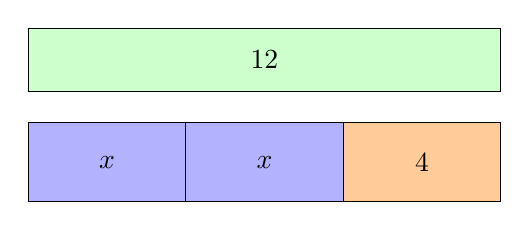
\begin{tikzpicture}
  \draw[fill=blue!30] (0,0) rectangle (2,1) node[midway] {$x$};
  \draw[fill=blue!30] (2,0) rectangle (4,1) node[midway] {$x$};
  \draw[fill=orange!40] (4,0) rectangle (6,1) node[midway] {$4$};
  \draw[fill=green!20] (0,1.4) rectangle (6,2.2) node[midway] {$12$};
\end{tikzpicture}
\end{center}

\begin{itemize}
  \item Write an equation represented by the bar model and solve it. \ashow{$2x+4=12$, so $x=4$.}
  \item If the total was 18 instead of 12, what would $x$ be\ashowq{~$x=7$.}
  \item Is $3(x+4)=3x+4$ true or false? Explain. \ashow{False, because $3(x+4)=3x+12$.}
\end{itemize}

\end{frame}

%------------------------------------------------
\begin{frame}{Worked Solution: Starter 1, Question 1}
\hypertarget{work-st1}{}

\textbf{Question:} Calculate $-5+12=$\ablank{$7$}.

\textbf{Worked Solution:} \ashow{Start at $-5$ and move $12$ units to the right, landing on $7$.}

\end{frame}

%------------------------------------------------
\begin{frame}{Worked Solution: Starter 1, Question 2}

\textbf{Question:} Collect like terms: $3x+4x=$\ablank{$7x$}.

\textbf{Worked Solution:} \ashow{Add the coefficients: $3+4=7$, so $3x+4x=7x$.}

\end{frame}

%------------------------------------------------
\begin{frame}{Worked Solution: Starter 1, Question 3}

\textbf{Question:} Expand: $3(x+4)=$\ablank{$3x+12$}.

\textbf{Worked Solution:} \ashow{Multiply each term inside the bracket by $3$: $3(x+4)=3x+12$.}

\end{frame}

%------------------------------------------------
\begin{frame}{Worked Solution: Starter 1, Question 4}

\textbf{Question:} Solve: $x+6=14 \Rightarrow$\ablank{$x=8$}.

\textbf{Worked Solution:} \ashow{Subtract $6$ from both sides: $x=14-6=8$.}

\end{frame}

%------------------------------------------------
\begin{frame}{Worked Solution: Starter 1, Question 5}

\textbf{Question:} Write an equation represented by the bar model and solve it.

\textbf{Worked Solution:} \ashow{The two $x$-blocks and the $4$-block make the total $12$, so $2x+4=12$. Subtract $4$: $2x=8$; divide by $2$: $x=4$.}

\end{frame}

%------------------------------------------------
\begin{frame}{Worked Solution: Starter 1, Question 6}

\textbf{Question:} If the total was 18 instead of 12, what would $x$ be\ashowq{~$x=7$.}

\textbf{Worked Solution:} \ashow{The model becomes $2x+4=18$. Subtract $4$: $2x=14$, so $x=7$.}

\end{frame}

%------------------------------------------------
\begin{frame}{Worked Solution: Starter 1, Question 7}

\textbf{Question:} Is $3(x+4)=3x+4$ true or false? Explain.

\textbf{Worked Solution:} \ashow{False. Expanding $3(x+4)$ gives $3x+12$, not $3x+4$.}

\end{frame}

%------------------------------------------------
\begin{frame}{Starter 2}
\hypertarget{q-st2}{}

\begin{itemize}
  \item Calculate: $6-11 =$ \ablank{$-5$}
  \item Collect like terms: $5x + 2 + 3x =$ \ablank{$8x+2$}
  \item Expand: $4(a + 2) =$ \ablank{$4a+8$}
  \item Solve: $2x = 14 \Rightarrow$ \ablank{$x=7$}
\end{itemize}

\vspace{0.3cm}

\begin{center}
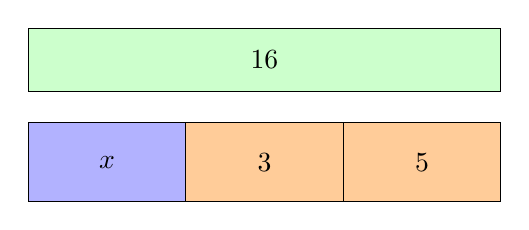
\begin{tikzpicture}
  \draw[fill=blue!30] (0,0) rectangle (2,1) node[midway] {$x$};
  \draw[fill=orange!40] (2,0) rectangle (4,1) node[midway] {$3$};
  \draw[fill=orange!40] (4,0) rectangle (6,1) node[midway] {$5$};
  \draw[fill=green!20] (0,1.4) rectangle (6,2.2) node[midway] {$16$};
\end{tikzpicture}
\end{center}

\begin{itemize}
  \item Write the equation represented by the bar model and solve it. \ashow{$x+3+5=16$, so $x=8$.}
  \item Which part of the diagram represents the constant? \ashow{The $3$ and $5$ blocks (total $8$).}
  \item Create a bar model for $8x + 2 = 26$. \ashow{Eight $x$-blocks and a $2$-block, with total $26$.}
  \item Simplify: $ax + bx =$ \ablank{$(a+b)x$}
\end{itemize}

\end{frame}

%------------------------------------------------
\begin{frame}{Worked Solution: Starter 2, Question 1}
\hypertarget{work-st2}{}

\textbf{Question:} Calculate $6-11=$\ablank{$-5$}.

\textbf{Worked Solution:} \ashow{Start at $6$ and move $11$ units left: $6-11=-5$.}

\end{frame}

%------------------------------------------------
\begin{frame}{Worked Solution: Starter 2, Question 2}

\textbf{Question:} Collect like terms: $5x+2+3x=$\ablank{$8x+2$}.

\textbf{Worked Solution:} \ashow{Collect the $x$-terms: $5x+3x=8x$; keep the constant $+2$: $8x+2$.}

\end{frame}

%------------------------------------------------
\begin{frame}{Worked Solution: Starter 2, Question 3}

\textbf{Question:} Expand: $4(a+2)=$\ablank{$4a+8$}.

\textbf{Worked Solution:} \ashow{Multiply each term by $4$: $4(a+2)=4a+8$.}

\end{frame}

%------------------------------------------------
\begin{frame}{Worked Solution: Starter 2, Question 4}

\textbf{Question:} Solve: $2x=14 \Rightarrow$\ablank{$x=7$}.

\textbf{Worked Solution:} \ashow{Divide both sides by $2$: $x=\frac{14}{2}=7$.}

\end{frame}

%------------------------------------------------
\begin{frame}{Worked Solution: Starter 2, Question 5}

\textbf{Question:} Write the equation represented by the bar model and solve it.

\textbf{Worked Solution:} \ashow{The bar model has $x+3+5=16$. Since $3+5=8$, we get $x+8=16$, so $x=8$.}

\end{frame}

%------------------------------------------------
\begin{frame}{Worked Solution: Starter 2, Question 6}

\textbf{Question:} Which part of the diagram represents the constant?

\textbf{Worked Solution:} \ashow{The $3$ and $5$ blocks have no $x$, so together they represent the constant $8$.}

\end{frame}

%------------------------------------------------
\begin{frame}{Worked Solution: Starter 2, Question 7}

\textbf{Question:} Create a bar model for $8x + 2 = 26$.

\textbf{Worked Solution:} \ashow{Draw eight equal $x$-blocks and one $2$-block, with total $26$.}

\begin{center}
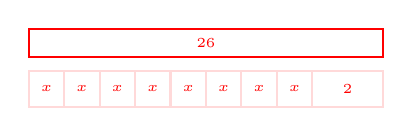
\begin{tikzpicture}[scale=0.45]
  \draw[ans, ansfill] (0,0) rectangle (1,1) node[midway, anslab] {$x$};
  \draw[ans, ansfill] (1,0) rectangle (2,1) node[midway, anslab] {$x$};
  \draw[ans, ansfill] (2,0) rectangle (3,1) node[midway, anslab] {$x$};
  \draw[ans, ansfill] (3,0) rectangle (4,1) node[midway, anslab] {$x$};
  \draw[ans, ansfill] (4,0) rectangle (5,1) node[midway, anslab] {$x$};
  \draw[ans, ansfill] (5,0) rectangle (6,1) node[midway, anslab] {$x$};
  \draw[ans, ansfill] (6,0) rectangle (7,1) node[midway, anslab] {$x$};
  \draw[ans, ansfill] (7,0) rectangle (8,1) node[midway, anslab] {$x$};
  \draw[ans, ansfill] (8,0) rectangle (10,1) node[midway, anslab] {$2$};
  \draw[ans] (0,1.4) rectangle (10,2.2) node[midway, anslab] {$26$};
\end{tikzpicture}
\end{center}

\end{frame}

%------------------------------------------------
\begin{frame}{Worked Solution: Starter 2, Question 8}

\textbf{Question:} Simplify: $ax+bx=$\ablank{$(a+b)x$}.

\textbf{Worked Solution:} \ashow{Factor out the common $x$: $ax+bx=(a+b)x$.}

\end{frame}

%------------------------------------------------
\begin{frame}{Starter 3}
\hypertarget{q-st3}{}

\begin{itemize}
  \item Calculate: $-3 + 8 =$ \ablank{$5$}
  \item Collect like terms: $6a + 3 + 2a =$ \ablank{$8a+3$}
  \item Expand: $2(x + 7) =$ \ablank{$2x+14$}
  \item Solve: $x - 4 = 9 \Rightarrow$ \ablank{$x=13$}
\end{itemize}

\vspace{0.3cm}

\begin{center}
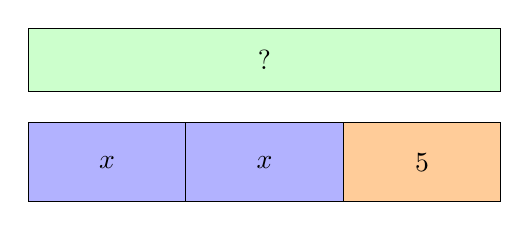
\begin{tikzpicture}
  \draw[fill=blue!30] (0,0) rectangle (2,1) node[midway] {$x$};
  \draw[fill=blue!30] (2,0) rectangle (4,1) node[midway] {$x$};
  \draw[fill=orange!40] (4,0) rectangle (6,1) node[midway] {$5$};
  \draw[fill=green!20] (0,1.4) rectangle (6,2.2) node[midway] {$?$};
\end{tikzpicture}
\end{center}

\begin{itemize}
  \item Suppose the total is 17. Write and solve the equation. \ashow{$2x+5=17$, so $x=6$.}
  \item Suppose the total is 25. What is $x$ now\ashowq{~$x=10$.}
  \item Expand: $3(x+7) =$ \ablank{$3x+21$}
  \item Expand: $3(x-7) =$ \ablank{$3x-21$}
\end{itemize}

\end{frame}

%------------------------------------------------
\begin{frame}{Worked Solution: Starter 3, Question 1}
\hypertarget{work-st3}{}

\textbf{Question:} Calculate $-3+8=$\ablank{$5$}.

\textbf{Worked Solution:} \ashow{Start at $-3$ and move $8$ units right: $-3+8=5$.}

\end{frame}

%------------------------------------------------
\begin{frame}{Worked Solution: Starter 3, Question 2}

\textbf{Question:} Collect like terms: $6a+3+2a=$\ablank{$8a+3$}.

\textbf{Worked Solution:} \ashow{Collect $a$-terms: $6a+2a=8a$; keep $+3$: $8a+3$.}

\end{frame}

%------------------------------------------------
\begin{frame}{Worked Solution: Starter 3, Question 3}

\textbf{Question:} Expand: $2(x+7)=$\ablank{$2x+14$}.

\textbf{Worked Solution:} \ashow{Multiply each term by $2$: $2(x+7)=2x+14$.}

\end{frame}

%------------------------------------------------
\begin{frame}{Worked Solution: Starter 3, Question 4}

\textbf{Question:} Solve: $x-4=9 \Rightarrow$\ablank{$x=13$}.

\textbf{Worked Solution:} \ashow{Add $4$ to both sides: $x=9+4=13$.}

\end{frame}

%------------------------------------------------
\begin{frame}{Worked Solution: Starter 3, Question 5}

\textbf{Question:} Suppose the total is 17. Write and solve the equation.

\textbf{Worked Solution:} \ashow{The model has two $x$-blocks and a $5$-block, so $2x+5=17$. Subtract $5$: $2x=12$, so $x=6$.}

\end{frame}

%------------------------------------------------
\begin{frame}{Worked Solution: Starter 3, Question 6}

\textbf{Question:} Suppose the total is 25. What is $x$ now\ashowq{~$x=10$.}

\textbf{Worked Solution:} \ashow{Now $2x+5=25$. Subtract $5$: $2x=20$, so $x=10$.}

\end{frame}

%------------------------------------------------
\begin{frame}{Worked Solution: Starter 3, Question 7}

\textbf{Question:} Expand: $3(x+7)=$\ablank{$3x+21$}.

\textbf{Worked Solution:} \ashow{$3(x+7)=3x+21$.}

\end{frame}

%------------------------------------------------
\begin{frame}{Worked Solution: Starter 3, Question 8}

\textbf{Question:} Expand: $3(x-7)=$\ablank{$3x-21$}.

\textbf{Worked Solution:} \ashow{$3(x-7)=3x+3(-7)=3x-21$.}

\end{frame}

%------------------------------------------------
\begin{frame}{Starter 4}
\hypertarget{q-st4}{}

\begin{itemize}
  \item Calculate: $-6 \div 3 =$ \ablank{$-2$}
  \item Collect like terms: $9a - 4a + 2 + 3b =$ \ablank{$5a+2+3b$}
  \item Expand: $5(y + 3) =$ \ablank{$5y+15$}
  \item Solve: $3d = 18 \Rightarrow$ \ablank{$d=6$}
\end{itemize}

\vspace{0.3cm}

\begin{center}
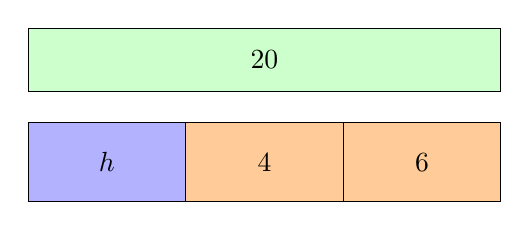
\begin{tikzpicture}
  \draw[fill=blue!30] (0,0) rectangle (2,1) node[midway] {$h$};
  \draw[fill=orange!40] (2,0) rectangle (4,1) node[midway] {$4$};
  \draw[fill=orange!40] (4,0) rectangle (6,1) node[midway] {$6$};
  \draw[fill=green!20] (0,1.4) rectangle (6,2.2) node[midway] {$20$};
\end{tikzpicture}
\end{center}

\begin{itemize}
  \item Write an equation represented by the diagram and solve for $h$. \ashow{$h+4+6=20$, so $h=10$.}
  \item If the $4$ block was instead $h$ and the $h$ block was $4$, what equation would we have\ashowq{~$4+h+6=20$.}
  \item Expand: $(x-3)(x-2) =$ \ablank{$x^2-5x+6$}
  \item Simplify: $a^2 \times a \times b =$ \ablank{$a^3b$}
\end{itemize}

\end{frame}

%------------------------------------------------
\begin{frame}{Worked Solution: Starter 4, Question 1}
\hypertarget{work-st4}{}

\textbf{Question:} Calculate $-6 \div 3=$\ablank{$-2$}.

\textbf{Worked Solution:} \ashow{Dividing $-6$ into three equal groups gives $-2$; check: $3\times(-2)=-6$.}

\end{frame}

%------------------------------------------------
\begin{frame}{Worked Solution: Starter 4, Question 2}

\textbf{Question:} Collect like terms: $9a-4a+2+3b=$\ablank{$5a+2+3b$}.

\textbf{Worked Solution:} \ashow{$9a-4a=5a$; the constant $2$ and the $b$-term $3b$ stay separate, so $5a+2+3b$.}

\end{frame}

%------------------------------------------------
\begin{frame}{Worked Solution: Starter 4, Question 3}

\textbf{Question:} Expand: $5(y+3)=$\ablank{$5y+15$}.

\textbf{Worked Solution:} \ashow{$5(y+3)=5y+5\cdot3=5y+15$.}

\end{frame}

%------------------------------------------------
\begin{frame}{Worked Solution: Starter 4, Question 4}

\textbf{Question:} Solve: $3d=18 \Rightarrow$\ablank{$d=6$}.

\textbf{Worked Solution:} \ashow{Divide both sides by $3$: $d=18/3=6$.}

\end{frame}

%------------------------------------------------
\begin{frame}{Worked Solution: Starter 4, Question 5}

\textbf{Question:} Write an equation represented by the diagram and solve for $h$.

\textbf{Worked Solution:} \ashow{The diagram gives $h+4+6=20$, so $h+10=20$, hence $h=10$.}

\end{frame}

%------------------------------------------------
\begin{frame}{Worked Solution: Starter 4, Question 6}

\textbf{Question:} If the $4$ block was instead $h$ and the $h$ block was $4$, what equation would we have\ashowq{~$4+h+6=20$.}

\textbf{Worked Solution:} \ashow{After swapping the labels, the equation is $4+h+6=20$, which still gives $h=10$.}

\end{frame}

%------------------------------------------------
\begin{frame}{Worked Solution: Starter 4, Question 7}

\textbf{Question:} Expand: $(x-3)(x-2)=$\ablank{$x^2-5x+6$}.

\textbf{Worked Solution:} \ashow{Use FOIL: $x^2-2x-3x+6=x^2-5x+6$.}

\end{frame}

%------------------------------------------------
\begin{frame}{Worked Solution: Starter 4, Question 8}

\textbf{Question:} Simplify: $a^2 \times a \times b=$\ablank{$a^3b$}.

\textbf{Worked Solution:} \ashow{Combine the powers of $a$: $a^2\times a=a^3$, then multiply by $b$: $a^3b$.}

\end{frame}

%------------------------------------------------
\begin{frame}{Starter 5}
\hypertarget{q-st5}{}

\begin{itemize}
  \item Calculate: $7 - 12 =$ \ablank{$-5$}
  \item Collect like terms: $2x + 7 + 3x =$ \ablank{$5x+7$}
  \item Expand: $3(a + 5) =$ \ablank{$3a+15$}
  \item Solve: $2x + 3 = 11 \Rightarrow$ \ablank{$x=4$}
\end{itemize}

\vspace{0.3cm}

\begin{center}
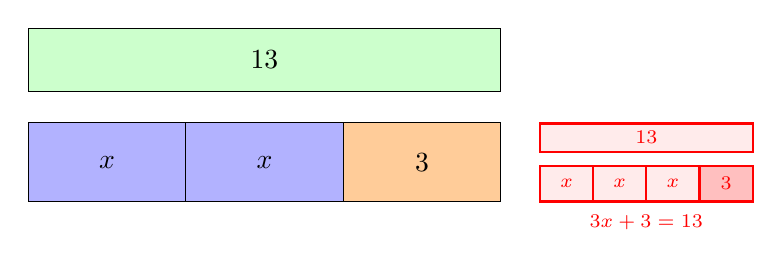
\begin{tikzpicture}
  \draw[fill=blue!30] (0,0) rectangle (2,1) node[midway] {$x$};
  \draw[fill=blue!30] (2,0) rectangle (4,1) node[midway] {$x$};
  \draw[fill=orange!40] (4,0) rectangle (6,1) node[midway] {$3$};
  \draw[fill=green!20] (0,1.4) rectangle (6,2.2) node[midway] {$13$};

% --- Q3 answer: a bar model for 3x + 3 = 13, drawn beside the given model ---
\begin{scope}[shift={(6.5,0)}, scale=0.45]
  \draw[ans, fill=red!8]  (0,1.4) rectangle (6,2.2)  node[midway, anslab, font=\scriptsize] {$13$};
  \draw[ans, fill=red!8]  (0,0) rectangle (1.5,1)    node[midway, anslab, font=\scriptsize] {$x$};
  \draw[ans, fill=red!8]  (1.5,0) rectangle (3,1)    node[midway, anslab, font=\scriptsize] {$x$};
  \draw[ans, fill=red!8]  (3,0) rectangle (4.5,1)    node[midway, anslab, font=\scriptsize] {$x$};
  \draw[ans, fill=red!25] (4.5,0) rectangle (6,1)    node[midway, anslab, font=\scriptsize] {$3$};
  \node[anslab, below, font=\scriptsize] at (3,-0.1) {$3x+3=13$};
\end{scope}
\end{tikzpicture}
\end{center}

\begin{itemize}
  \item Write and solve the equation represented by the model. \ashow{$2x+3=13$, so $x=5$.}
  \item Explain how each part of the diagram matches the equation. \ashow{Two $x$-blocks and a $3$-block make the total $13$.}
  \item Draw a bar model to represent $3x + 3 = 13$.
  \item Write an equation with solution $x=5$. \ashow{e.g.\ $x+2=7$.}
\end{itemize}

\end{frame}

%------------------------------------------------
\begin{frame}{Worked Solution: Starter 5, Question 1}
\hypertarget{work-st5}{}

\textbf{Question:} Calculate $7-12=$\ablank{$-5$}.

\textbf{Worked Solution:} \ashow{$7-12=-(12-7)=-5$.}

\end{frame}

%------------------------------------------------
\begin{frame}{Worked Solution: Starter 5, Question 2}

\textbf{Question:} Collect like terms: $2x+7+3x=$\ablank{$5x+7$}.

\textbf{Worked Solution:} \ashow{$2x+3x=5x$; keep $+7$: $5x+7$.}

\end{frame}

%------------------------------------------------
\begin{frame}{Worked Solution: Starter 5, Question 3}

\textbf{Question:} Expand: $3(a+5)=$\ablank{$3a+15$}.

\textbf{Worked Solution:} \ashow{$3(a+5)=3a+15$.}

\end{frame}

%------------------------------------------------
\begin{frame}{Worked Solution: Starter 5, Question 4}

\textbf{Question:} Solve: $2x+3=11 \Rightarrow$\ablank{$x=4$}.

\textbf{Worked Solution:} \ashow{Subtract $3$: $2x=8$; divide by $2$: $x=4$.}

\end{frame}

%------------------------------------------------
\begin{frame}{Worked Solution: Starter 5, Question 5}

\textbf{Question:} Write and solve the equation represented by the model.

\textbf{Worked Solution:} \ashow{The model shows $2x+3=13$. Subtract $3$: $2x=10$, so $x=5$.}

\end{frame}

%------------------------------------------------
\begin{frame}{Worked Solution: Starter 5, Question 6}

\textbf{Question:} Explain how each part of the diagram matches the equation.

\textbf{Worked Solution:} \ashow{Two $x$-blocks give $2x$, the $3$-block is the constant $3$, and the total $13$ is written above them.}

\end{frame}

%------------------------------------------------
\begin{frame}{Worked Solution: Starter 5, Question 7}

\textbf{Question:} Draw a bar model to represent $3x+3=13$.

\textbf{Worked Solution:} \ashow{Use three equal $x$-blocks, a $3$-block, and total $13$.}

\begin{center}
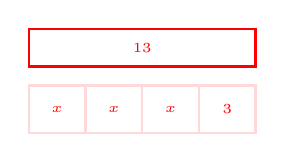
\begin{tikzpicture}[scale=0.6]
  \draw[ans, ansfill] (0,0) rectangle (1.2,1) node[midway, anslab] {$x$};
  \draw[ans, ansfill] (1.2,0) rectangle (2.4,1) node[midway, anslab] {$x$};
  \draw[ans, ansfill] (2.4,0) rectangle (3.6,1) node[midway, anslab] {$x$};
  \draw[ans, ansfill] (3.6,0) rectangle (4.8,1) node[midway, anslab] {$3$};
  \draw[ans] (0,1.4) rectangle (4.8,2.2) node[midway, anslab] {$13$};
\end{tikzpicture}
\end{center}

\end{frame}

%------------------------------------------------
\begin{frame}{Worked Solution: Starter 5, Question 8}

\textbf{Question:} Write an equation with solution $x=5$.

\textbf{Worked Solution:} \ashow{One example is $x+2=7$, because $5+2=7$. Many equations work.}

\end{frame}

%------------------------------------------------
\begin{frame}{Starter 6}
\hypertarget{q-st6}{}

\begin{itemize}
  \item Calculate: $-4 \times 6 =$ \ablank{$-24$}
  \item Collect like terms: $7x + 3x - 5 =$ \ablank{$10x-5$}
  \item Expand: $2(3x + 4) =$ \ablank{$6x+8$}
  \item Solve: $3x + 5 = 17 \Rightarrow$ \ablank{$x=4$}
\end{itemize}

\vspace{0.2cm}

\begin{itemize}
  \item Solve: $4x + 3 = 2x + 15 \Rightarrow$ \ablank{$x=6$}
  \item Solve: $\frac{x}{3} + 4 = 9 \Rightarrow$ \ablank{$x=15$}
\end{itemize}

\vspace{0.3cm}

\begin{center}
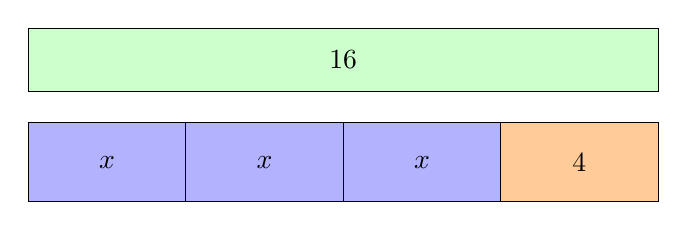
\begin{tikzpicture}

  \draw[fill=blue!30] (0,0) rectangle (2,1) node[midway] {$x$};
  \draw[fill=blue!30] (2,0) rectangle (4,1) node[midway] {$x$};
  \draw[fill=blue!30] (4,0) rectangle (6,1) node[midway] {$x$};
  \draw[fill=orange!40] (6,0) rectangle (8,1) node[midway] {$4$};
  \draw[fill=green!20] (0,1.4) rectangle (8,2.2) node[midway] {$16$};

\end{tikzpicture}
\end{center}

\begin{itemize}
  \item Write one equation that could be represented by this bar model. \ashow{$3x+4=16$.}
  \item Write a different equation with the same solution. \ashow{e.g.\ $2x+3=11$.}
  \item Create an equation with solution $x=4$ that includes a negative term. \ashow{e.g.\ $2x-3=5$.}
\end{itemize}

\end{frame}

%------------------------------------------------
\begin{frame}{Worked Solution: Starter 6, Question 1}
\hypertarget{work-st6}{}

\textbf{Question:} Calculate $-4 \times 6=$\ablank{$-24$}.

\textbf{Worked Solution:} \ashow{$4\times6=24$, and one negative factor makes the product negative: $-24$.}

\end{frame}

%------------------------------------------------
\begin{frame}{Worked Solution: Starter 6, Question 2}

\textbf{Question:} Collect like terms: $7x+3x-5=$\ablank{$10x-5$}.

\textbf{Worked Solution:} \ashow{$7x+3x=10x$, so $10x-5$.}

\end{frame}

%------------------------------------------------
\begin{frame}{Worked Solution: Starter 6, Question 3}

\textbf{Question:} Expand: $2(3x+4)=$\ablank{$6x+8$}.

\textbf{Worked Solution:} \ashow{$2(3x+4)=6x+8$.}

\end{frame}

%------------------------------------------------
\begin{frame}{Worked Solution: Starter 6, Question 4}

\textbf{Question:} Solve: $3x+5=17 \Rightarrow$\ablank{$x=4$}.

\textbf{Worked Solution:} \ashow{Subtract $5$: $3x=12$; divide by $3$: $x=4$.}

\end{frame}

%------------------------------------------------
\begin{frame}{Worked Solution: Starter 6, Question 5}

\textbf{Question:} Solve: $4x+3=2x+15 \Rightarrow$\ablank{$x=6$}.

\textbf{Worked Solution:} \ashow{Subtract $2x$ from both sides: $2x+3=15$. Subtract $3$: $2x=12$; divide by $2$: $x=6$.}

\end{frame}

%------------------------------------------------
\begin{frame}{Worked Solution: Starter 6, Question 6}

\textbf{Question:} Solve: $\frac{x}{3}+4=9 \Rightarrow$\ablank{$x=15$}.

\textbf{Worked Solution:} \ashow{Subtract $4$: $\frac{x}{3}=5$; multiply by $3$: $x=15$.}

\end{frame}

%------------------------------------------------
\begin{frame}{Worked Solution: Starter 6, Question 7}

\textbf{Question:} Write one equation that could be represented by this bar model.

\textbf{Worked Solution:} \ashow{The model has three $x$-blocks and a $4$-block with total $16$, so $3x+4=16$.}

\end{frame}

%------------------------------------------------
\begin{frame}{Worked Solution: Starter 6, Question 8}

\textbf{Question:} Write a different equation with the same solution.

\textbf{Worked Solution:} \ashow{Since $3x+4=16$ gives $x=4$, a different equation is $2x+3=11$, which also gives $x=4$.}

\end{frame}

%------------------------------------------------
\begin{frame}{Worked Solution: Starter 6, Question 9}

\textbf{Question:} Create an equation with solution $x=4$ that includes a negative term.

\textbf{Worked Solution:} \ashow{For example, $2x-3=5$: adding $3$ gives $2x=8$, so $x=4$.}

\end{frame}

%------------------------------------------------
\end{document}